 \section{Komponenten}
 
 \subsection{Verknüpfung\label{Verknuepfung}}%
Die Verknüpfung der Komponenten erfolgt zentral aus der Datenbank heraus, dort gibt es die Tabelle $Component$ und $ComponentLinkage$, diese definieren die Orte der Komponenten und die Verknüpfung derer. Dabei können lediglich Aufrufe definiert werden. Ein $Link$ zwischen zwei Komponenten A, als Besitzer des Links und B als Ziel des Links, stellt damit einen Aufruf von A nach B dar.

Beispiele für eine solche Verknüpfung befinden sich in der Datei \blau{DB/Components.sql}.
Diese sind fest für die Datenbank $uebungsplattform$ angelegt, sofern Sie eine andere Datenbank nutzen möchten, ändern Sie diese Bezeichnung.

\begin{minipage}{\textwidth}
Beispiel eines Komponenteneintrages der Tabelle $Component$
\begin{lstlisting}
...
INSERT INTO `uebungsplattform`.`Component` 
(`CO_id`, `CO_name`, `CO_address`, `CO_option`) VALUES 
(1, 'FSControl', 'localhost/uebungsplattform/FS/FSControl', '');
...
\end{lstlisting}
\end{minipage}

\begin{minipage}{\textwidth}
Beispiel eines Verlinkungseintrages der Tabelle $ComponentLinkage$
\begin{lstlisting}
...
INSERT INTO `uebungsplattform`.`ComponentLinkage` 
(`CL_id`, `CO_id_owner`, `CL_name`, `CL_relevanz`, `CO_id_target`) 
VALUES (1, 3, 'getFile', '', 1);
...
\end{lstlisting}
\end{minipage}


Dazu wurde eine Komponente $CControl$ in \blau{DB/CControl} entwickelt. Diese stellt Funktionen bereit, um die Definitionen in die Datenbank einzutragen und zu entnehmen.

Mit Hilfe des Aufrufs \blau{DB/CControl/send} entnimmt die Komponente CControl die Definitionen aus der DB und versendet sie an alle betroffenen Komponenten. 

Die Ausgabe eines solchen Aufrufs könnte folgendermaßen aussehen: \\
\blau{201--FSControl--localhost/uebungsplattform/FS/FSControl}\\
\blau{201--FSFile--localhost/uebungsplattform/FS/FSFile}\\
\blau{201--FSZip--localhost/uebungsplattform/FS/FSZip}\\
\blau{201--DBControl--localhost/uebungsplattform/DB/DBControl}\\
\blau{201--FSBinder--localhost/uebungsplattform/FS/FSBinder}\\
...\\

Dabei stehen links die HTTP Statuscodes der Antworten der Komponenten, mittig der Name der Komponenten aus der Datenbank und rechts die Adresse, welcher die Definition geschickt wurde.

Dabei nehmen die Komponenten diese Informationen entgegen und legen in ihrem Ordner \blau{CConfig.json} Dateien an.
Diese Enthalten die Informationen über die Komponenten selbst und die Informationen über die definierten Links.

\begin{minipage}{\textwidth}
\begin{lstlisting}
{
    "id": "6",
    "name": "DBCourse",
    "address": "localhost/uebungsplattform/DB/DBCourse",
    "option": "",
    "prefix": "course",
    "links": [
        {
            "id": "6",
            "name": "out",
            "address": "localhost/uebungsplattform/DB/DBQuery",
            "target": "13",
            "prefix": "query",
            "owner": "6",
            "relevanz": ""
        }
    ]
}
\end{lstlisting}
\end{minipage}

Diese Informationen können mit der, in der Datei \blau{Assistants/CConfig.php} definierten Klasse $CConfig$ in der Komponenten genutzt werden.
Dazu sollte am besten noch vor dem Aufrufen der eigentlichen Komponente ein Objekt dieser Klasse erstellt und mit entsprechenden Informationen versorgt werden. So kann jede Komponente für sich einen Präfix vergeben, auf den sie reagiert. Sollte sie keinen bestimmten Präfix verlangen, so wird ein leerer String '' angegeben, bei der Nutzung mehrerer werden diese durch Komma getrennt.

Das CConfig Objekt enthält selber einen Slim Aufruf, der prüft ob die Komponente mit $/component$ aufgerufen wurde, in diesem Falle würde die Komponente mit eingehenden Definitionsdaten oder dem Abrufen derer rechnen.

Um die Verknüpfung in einer Komponente umzusetzen, könnte man folgendermaßen vorgehen.

\begin{minipage}{\textwidth}
\begin{lstlisting}
include_once( '../../Assistants/CConfig.php' );
...
// erstellt das CConfig Objekt und teilt allen anderen mit,
// dass diese Komponenten auf den Praefix course reagiert
$com = new CConfig(course);

// Wenn es keinen '/component' Aufruf gab, kann die eigentliche
// Komponente DBCourse geladen werden.
if (!$com->used())
    new DBCourse());
  
\end{lstlisting}
\end{minipage}

Möchte man nun die Links in seiner Komponente nutzen, so müssen sie zunächst aus der \blau{CConfig.json} geladen werden mit \blau{\$com-$>$loadConfig()}.

\begin{minipage}{\textwidth}
\begin{lstlisting}
...
// laedt die CConfig.json
$conf = $com->loadConfig() ;

// laedt ein Array von Link Objekten in $links
$links = $conf->getLinks(); 
\end{lstlisting}
\end{minipage}

Weitere Informationen über den Aufbau der Component und der Link Datenstruktur können den \blau{Assistants/Structures/Component.php} und \blau{Assistants/Structures/Link.php} Dateien entnommen werden.

Wichtig ist noch zu wissen, dass die Komponenten, wenn sie die Definitionen empfangen haben, nicht wissen, welchen Präfixe die Komponenten besitzen, mit denen sie verknüpft sind. Dazu werden sie bei jedem Aufruf prüfen, ob sie alle Präfixe kennen und in dem Fall, in dem sie einen Präfix nicht kennen, diesen von der entsprechenden Komponente abfragen.

Sollte es also zu langen Wartezeiten beim Aufrufen von Komponenten kommen, sollte geprüft werden, ob die Komponente alle ihre Ziele erreichen kann oder sie eventuell vergebens versucht diese zu kontaktieren.

 \subsection{Testen}
 Für den größten Teil der Komponenten wurden einfache Tests entwickelt, um PHP Syntaxfehler zu verhindern. 
 
  \subsubsection{Dateien}
 \begin{tabular}{l>{$}r<{$}}

\multirow{7}{.20\textwidth}{Database.sql} & \multirow{7}{.70\textwidth}{Enthält die aus \blau{Database.mwb} generierte SQL Datenbankdefinition. Diese Datei erstellt eine Datenbank mit dem Namen $uebungsplattform$, sofern eine solche Datenbank bereits existiert, wird die bereits existierende zuvor entfernt. Das einspielen erfolgt über die Konsole nach dem einloggen bei $mysql$ mittels \blau{source Database.sql} oder mit Hilfe von PHPMyAdmin, über $import$.}\\&\\&\\& \\&\\&\\&\\\hline

\multirow{7}{.20\textwidth}{Insert.sql} & \multirow{7}{.70\textwidth}{Enthält Beispieldaten für die Datenbank, diese werden auch für die Testszenarien genutzt. Das einspielen erfolgt entweder überden PHPMyAdmin mit $import$ oder über die Konsole mit \blau{mysql uebungsplattform $<$ Insert.sql} (http://dev.mysql.com/doc/refman/5.0/en/mysql-batch-commands.html)}\\&\\& \\&\\&\\& \\&\\
 \end{tabular}
 
  Zusätzlich gibt es die Datei \blau{DB/Components.sql}, diese enthält Beispielverknüpfungen für die Datenbank $uebungsplattform$ und muss ebenfalls eingespielt oder aber abgeändert werden.
 
Zudem enthält jeder Komponentenordner eine Testklasse, welche entsprechend der Komponente mit dem Namenszusatz "Test" versehen ist (Bsp. DBUserTest.php) und eine Definitionsdatei für phpunit selbst (phpunit.xml), in diesen Ordnern.

  \begin{minipage}[b]{1\linewidth}
    \centering
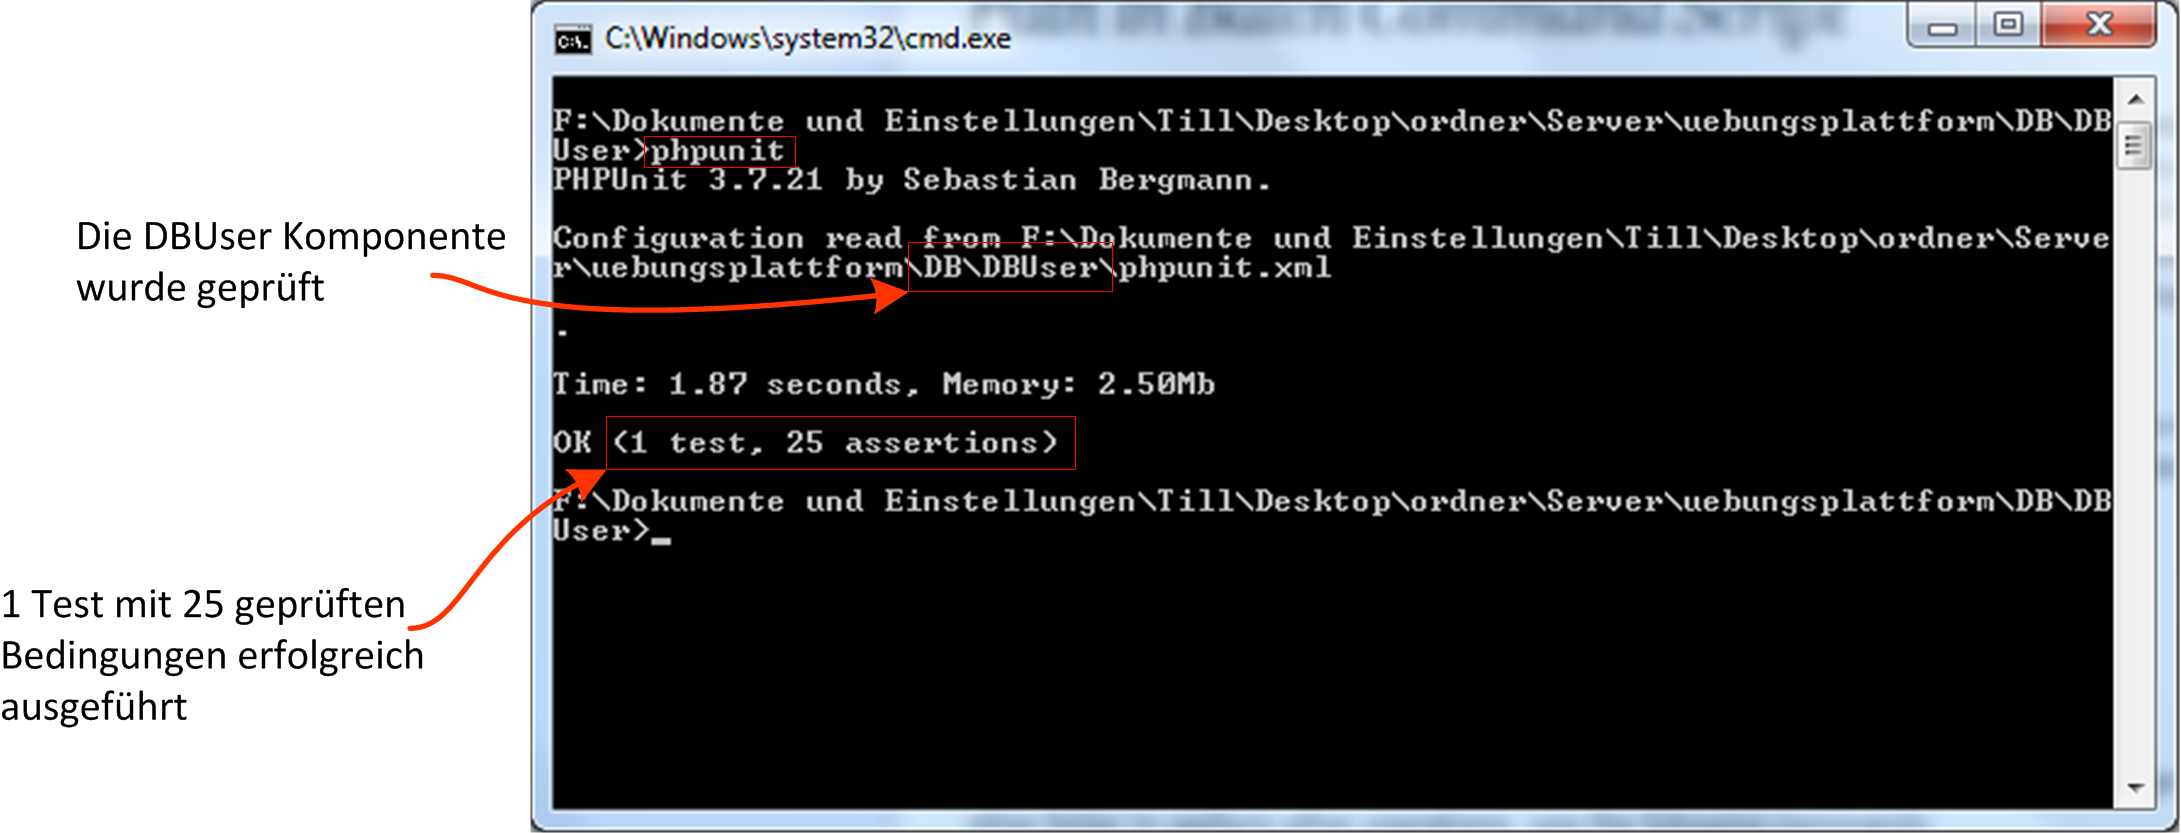
\includegraphics[scale=1]{Images/Testen.png}
  \end{minipage}\hfill

\subsubsection{Software}
  \begin{tabular}{l>{$}r<{$}}
\multirow{2}{.20\textwidth}{MySQL Server} & \multirow{2}{.70\textwidth}{Zum Betreiben der Datenbank (http://dev.mysql.com/downloads/mysql/)}\\& \\ \hline
\multirow{2}{.20\textwidth}{PHPUnit} & \multirow{2}{.70\textwidth}{Die Testumgebung (http://phpunit.de/)}\\&\\
 \end{tabular}

\subsubsection{Einstellungen}
Die Anfragegrundadresse für die HTTP Requests muss in der entsprechenden \blau{DB/phpunit.ini} eingestellt werden.

Beispielinhalt der \blau{phpunit.ini} Datei:

\begin{minipage}{\textwidth}
\begin{lstlisting}
[PHPUNIT]
// Die Anfrageadresse fuer die HTTP Requests
url = http://localhost/uebungsplattform/DB/ 
\end{lstlisting}
\end{minipage}
 
 \subsection{Der lange Weg zur neuen Komponente}
 \subsubsection{Entwickeln}
 Es muss sichergestellt werden, dass die Aufrufe dieser Komponente mittels REST möglich sind, dazu kann, sofern PHP zum Einsatz kommt, kann das Slim Framework genutzt werden, entsprechende Beispiele zur Nutzung können ebenfalls bereits bestehenden Komponenten entnommen werden. 
 
\begin{minipage}{\textwidth}
Beispiel:
\begin{lstlisting}
require_once( '../../Assistants/Slim/Slim.php' );
\Slim\Slim::registerAutoloader();
...
// initialisiert slim
$this->_app = new \Slim\Slim();

// Slim soll auf einen PUT Aufruf an diese Komponenten,
// mit der URI /course/:courseid die Funktion "editCourse"
// aufrufen und $courseid setzen.
// Bsp.: /course/1 oder /course/abc
$this->_app->put('/course/:courseid',
                 array($this,'editCourse'));
...

// hier wird die aufzurufende Funktion definiert
public function editCourse($courseid)
{
    ...
}
\end{lstlisting}
\end{minipage}

Daten, welche in die Komponenten hineingehen oder diese verlassen, sollten JSON kodiert sein. Dazu kann im Kapitel über Datenstrukturen nachgelesen werden.

Wir Antworten mit unserer Komponente nun indem wir mindestens den HTTP Statuscode und einen Body der Antwort setzen.

\begin{minipage}{\textwidth}
\begin{lstlisting}
public function editCourse($courseid)
{
    // setzt den Statuscode
    $this->_app->response->setStatus(201);

    // setzt den Inhalt der Antwort
    $this->_app->response->setBody('[]');
    
    // beendet diesen Aufruf sofort, gibt aber die 
    // festgelegte Antwort trotzdem zurueck
    $this->_app->stop();
}
\end{lstlisting}
\end{minipage}

Jede Komponente sollte so entworfen werden, das man sie komplett eigenständig betreiben kann, abgesehen von Hilfsdateien, welche sich mehrere Komponenten teilen.


 
 \subsubsection{Anbinden}
 Um die Komponente mit anderen zu verbinden müssen die entsprechenden Einträge in der Datenbank angelegt werden, dies kann entweder über die $CControl$ Komponente mittels entsprechender Kommunikation erfolgen oder über einen direkten Zugriff auf die Datenbanktabellen $Component$ und $ComponentLinkage$. 
 
Dabei muss ein neuer Eintrag für die Komponente in der $Component$ Tabelle erstellt werden, sodass sie eine ID erhält. Wollen wir nun die neue Komponente eine andere Aufrufen lassen können, so erstellen wir einen neuen $ComponentLinkage$ Eintrag und vermerken unsere neue ID dort als $CO\_id\_owner$, sowie die ID der Komponente die wir aufrufen können wollen als $CO\_id\_target$. Zudem wird der Linkname $CL\_name$ in der Komponente später genutzt um die Verwendung dieser Verknüpfung zu erklären oder verschiedene Ziele, sofern eine Komponente mehrere Ausgänge hat, zu unterscheiden.

So besitzen beispielsweise einige Komponenten Links mit dem Namen $Controller$ und wissen, damit, dass sie diese für Anfragen an einen Controller nutzen. Diese Namensvergabe ist jedoch Sache des Entwicklers der Komponente, es gibt dafür keine Festlegungen. Der häufigste Name ist dabei $out$, da meist kein besonderer Name benötigt wird.
 
Bei einer Änderung der Verknüpfungen sollten diese mit den unter Komponenten-Verknüpfung beschriebenen Schritten neu eingespielt werden.